\subsection{UC 15 - Telegram - Notifiche push}

	\begin{figure}[H]
		\centering
		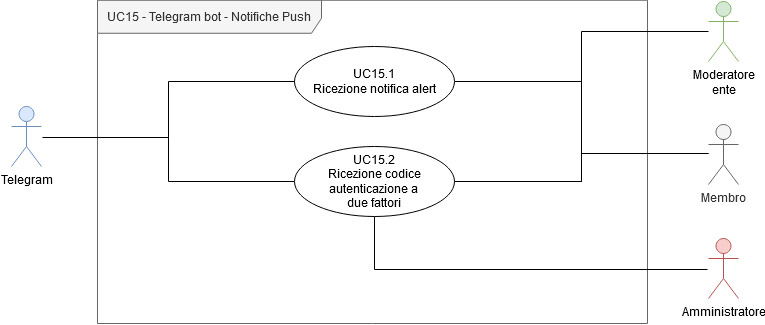
\includegraphics[scale=0.60]{res/images/uc15}
		\caption{Diagramma che descrive il processo notifica push tramite Telegram.}
	\end{figure}

	\begin{itemize}
		\item \textbf{attori primari:} membro, moderatore ente, amministratore;
		\item \textbf{attori secondari:} \glock{Telegram};
		\item \textbf{descrizione:} un utente, con l'applicazione di \glock{Telegram} attiva o in background, riceve una notifica push in base a un evento nel sistema;
		\item \textbf{precondizione:} l'utente ha l'applicazione di \glock{Telegram} attiva o in background e ha una chat autenticata con il \glock{bot};
		\item \textbf{postcondizione:} l'utente riceve una notifica da parte di \glock{Telegram};
		\item \textbf{scenario principale:}
		\begin{enumerate}
			\item l'utente ha l'applicazione di \glock{Telegram} attiva o in background;
			\item l'utente riceve una notifica push come messaggio di testo nella chat autorizzata con il \glock{bot}.
		\end{enumerate}
	\end{itemize}

	\subsubsection{UC 15.1 - Ricezione notifica alert}

	\begin{itemize}
		\item \textbf{attori primari:} membro, moderatore ente, amministratore;
		\item \textbf{attori secondari:} \glock{Telegram};
		\item \textbf{descrizione:} l'utente riceve una notifica sulla chat con il \glock{bot} di \glock{Telegram} relativa ad un \glock{alert} in cui un sensore ha superato una soglia prevista;
		\item \textbf{precondizione:} l'utente ha l'applicazione di \glock{Telegram} attiva o in background e ha una chat autenticata con il \glock{bot};
		\item \textbf{postcondizione:} l'utente riceve una notifica come messaggio di testo in chat con le informazioni relative all'\glock{alert};
		\item \textbf{scenario principale:}
		\begin{enumerate}
			\item l'utente ha l'applicazione di \glock{Telegram} attiva o in background;
			\item l'utente riceve una notifica che riguarda un \glock{alert} nella chat con il \glock{bot}.
		\end{enumerate}
	\end{itemize}

	\subsubsection{UC 15.2 - Ricezione codice di autenticazione a due fattori}

	\begin{itemize}
		\item \textbf{attori primari:} membro, moderatore ente, amministratore;
		\item \textbf{attori secondari:} \glock{Telegram};
		\item \textbf{descrizione:} l'utente riceve una notifica sulla chat con il \glock{bot} di \glock{Telegram} relativa al codice per l'autenticazione a due fattori, mentre sta svolgendo l'autenticazione nella \glock{web application};
		\item \textbf{precondizione:} l'utente ha l'applicazione di \glock{Telegram} attiva o in background e ha una chat autenticata con il \glock{bot};
		\item \textbf{postcondizione:} l'utente riceve una notifica come messaggio di testo in chat con le informazioni relative al codice per l'autenticazione a due fattori;
		\item \textbf{scenario principale:}
		\begin{enumerate}
			\item l'utente ha l'applicazione di \glock{Telegram} attiva o in background;
			\item l'utente riceve una notifica che riguarda il codice di autenticazione a due fattori da usare come credenziale per accedere alla \glock{web application}.
		\end{enumerate}
	\end{itemize}
